\chapter{PCB Design}
\thispagestyle{empty}
\label{chap13}

Printed Circuit Board (PCB) \index{PCB} design is an important
step in electronic system design. Every component of the circuit
needs to be placed and connections routed to minimise delay and
area. Each component has an associated footprint. Footprint refers to
the physical layout of a component that is required to mount it on the
PCB. PCB design involves associating footprints to all components, placing them appropriately to
minimise wire length and area, connecting the footprints using
tracks or vias and finally extracting the required files needed for
printing the PCB. Let us see the steps to design PCB using eSim. 

\section{Schematic creation for PCB design}
In \chapref{chap5}, we have seen the differences between schematic for
simulation and schematic for PCB design. Let us design a PCB Layout for a 'constant 5V DC supply'  circuit named as \texttt{7805VoltageRegulator}. First, we will simulate the circuit. Refer to \figref{pcbschfin} for the schematic used for simulation. After satisfying simulation results, we will move to PCB design. For this, we will remove the Source(s), Probes (plot\_v , plot\_db etc.), and global labels connected \texttt{solely} for the purpose of viewing simulation plots conveniently. \\  Connectors are the physical components that are used to interface/connect the board to external peripherals or sources.

\begin{figure}
\centering
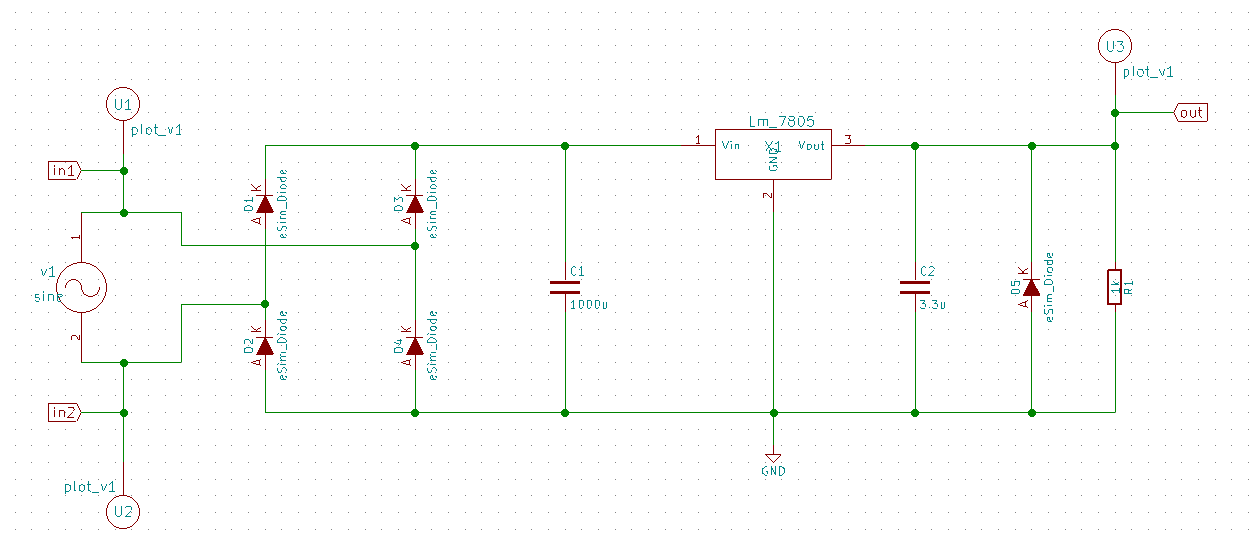
\includegraphics[width=\lgfig]{NGHDL/pcbschinitial.png}
\caption{Schematic for simulation of the constant 5V DC supply circuit}
\label{pcbschfin}
\end{figure}
 
%Create the circuit schematic as shown in \figref{pcbschfin}. The two pin female
%connector (\textt{Conn\_01x02\_Female}) can be placed from the Eeschema's \textt {Conn} library. Do the annotation and
%test for ERC.  Refer to \chapref{chap5} to know more about
%basic steps in schematic creation. 


\subsection{Removing components required for simulation from the schematic}
\begin{itemize}
\item We will remove the components which were placed for simulation purpose only.
\item Components that will be placed on the board need to be added in the schematic.
\item Modify the circuit schematic as shown in \figref{pcbschconn}. The two pin female connector (\texttt{Conn\_01x02\_Female}) is placed for the taking the 5V output supply meanwhile a 2 pin Screw Terminal (\texttt{Screw\_Terminal\_01x02}) is used to transmit the input signal on board. Do the annotation and test for ERC.  Refer to \chapref{chap5} to know more about basic steps in schematic creation. 

\begin{figure}
\centering
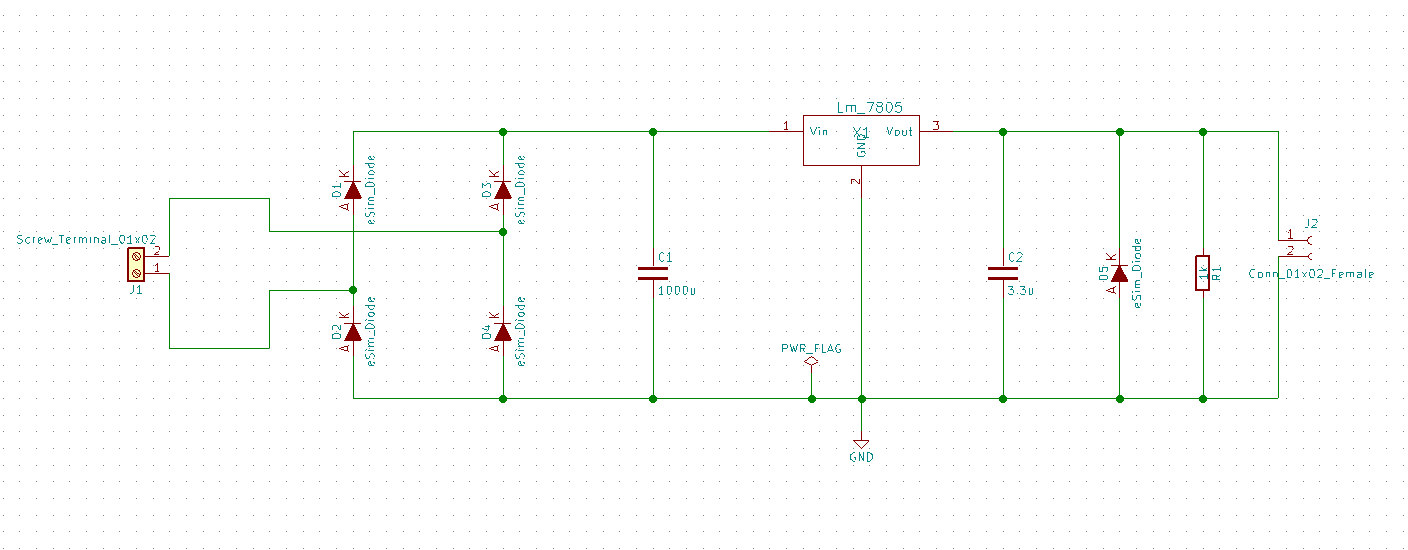
\includegraphics[width=\lgfig]{NGHDL/pcbschwithconn.png}
\caption{Schematic after adding connectors and removing the probes and sources.}
\label{pcbschconn}
\end{figure}
\end{itemize}

\subsection{Mapping of components using Cvpcb}
%\index{Footprints!mapping} \index{Footprint Editor}
\index{Component!footprint!mapping}
\begin{itemize}

\item Once the schematic for PCB Design is created, one needs to map each component
in the schematic to the appropriate footprint. The tool \texttt{Cvpcb} is
used for this.
\item Cvpcb can be launched by clicking the icon \texttt{Run Cvpcb to associate footprints and components} in Eeschema or by going under the \texttt{Tools} menu and selecting \texttt{Assign Component Footprint} option. 
\end{itemize}

\subsection{Familiarising with Cvpcb Window}
\index{Cvpcb}
\begin{itemize}
\item I. When one opens \texttt{Cvpcb} after annotating and running ERC on the schematic intended for PCB Design a window as shown in \figref{cvpcb} will be obtained. The Toolbar for using Cvpcb will be available in the top-most left corner.
\begin{figure}
\centering
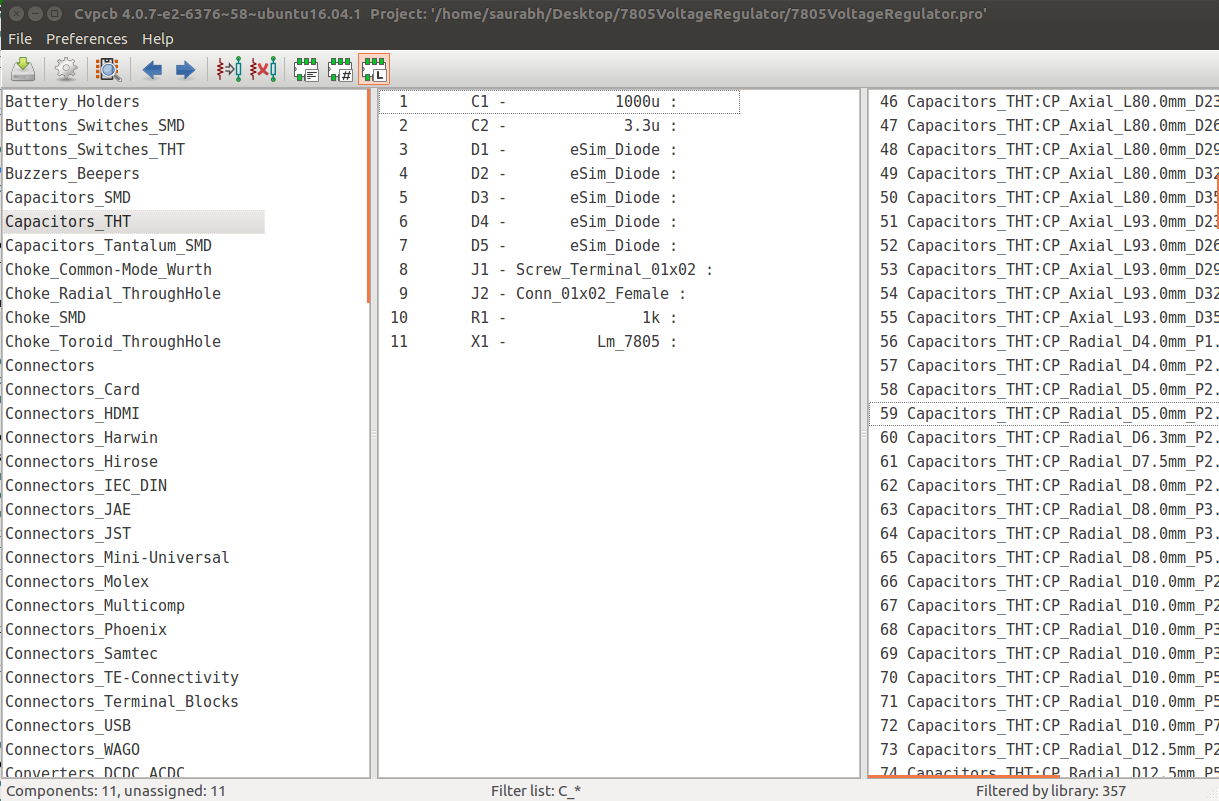
\includegraphics[width=\lgfig]{NGHDL/cvpcb_unassigned.png}
\caption{Cvpcb window}
\label{cvpcb}
\end{figure}
\item II. The left pane has a list of all footprint libraries in the database.
\item III. The middle pane displays the list of components present in the schematic and if any footprint is assigned/associated to them.
\item IV. The right pane has a list of available footprints for each component depending upon how of libraries.
\end{itemize}



\subsubsection{ Cvpcb Toolbar}
Some of the important tools in the toolbar are shown in
\figref{tb_fe}. They are explained below (Order of operation should ideally be from RIGHT to LEFT):
\begin{figure}
\centering

\includegraphics[width=\hgfig]{tb_fe.png}
\caption{Cvpcb Toolbar}
\label{tb_fe}
\end{figure}
\begin{compactenum}
\item Filter footprints list by library : We recommend the use of only this as a filtering method if you are completely new to eSim and/or PCB Design as it narrows down footprints based on libraries of the type of the component. When a filter is selected, it's icon will be highlighted in light red color as seen in \figref{tb_fe}.
\item Filter footprints list by pin count : This will filter the footprints based on number of pins the footprint has. This can be used to narrow down your search after sorting footprints by their library type.
\item Filter footprints list by keyword - This filters the footprints in the database based on keywords.
\item Automatic footprint association - Perform footprint association
  for each component automatically. Footprints will be selected from
  the list of footprints available.\\
  Note: This method of association is not recommended at all.
\item Delete all associations - Delete all the footprint associations made. This will erase all your association till now so be very careful in selecting this.
 \item Select next unlinked component: Using this you can go to the next component in the list of components for associating a footprint.
 \item Select previous unlinked component: Using this you can go to the previous component in the list of components for associating a footprint.
\item View selected footprint - View the selected footprint in 2D. See \secref{viewfp} for more details. \\
  Before clicking on this, make sure that a footprint is selected. Order of this operation should be
  \\ 1. Selection of footprint library from the left-most pane 
  \\ 2. Selecting a footprint from the right-most pane
  \\ 3. Click on \texttt{View selected footprint}
\item Edit footprint library table - One should familiarize themselves with Cvpcb first and then only choose to use this. This impacts the footprints that you can choose, so be careful before making any severe changes.
\item Save netlist and footprint files - Save the netlist and the
  footprints that are associated with it. One ought to save the association after having assigned proper footprints to all the components.
\end{compactenum}

\subsection{Viewing footprints in 2D and 3D}
\index{Footprints!view!2D}
\index{Footprints!view!3D}
\label{viewfp}

\begin{itemize}

\item To view a footprint in 2D, select the component for which you wish to view the available footprints, then select the library from left-most pane and now from the right pane and click on the desired footprint and click on \texttt{View selected footprint} from the menu bar. 
Let us view a footprint for \texttt{C1} from the \texttt{Capacitors\_THT} footprint library. Choose C1 from the middle pane as shown, click on \texttt{Capacitors\_THT} in the left-most pane and select the  
\textit{View selected footprint} tool.
On clicking the \textbf{View selected footprint} tool, the {\tt Footprint} window with the view in 2D will be displayed. 2D view of the footprint \texttt{CP\_Radial\_D5.0mm\_P2.50mm} is shown in \figref{2dview}.

\begin{figure}
\centering
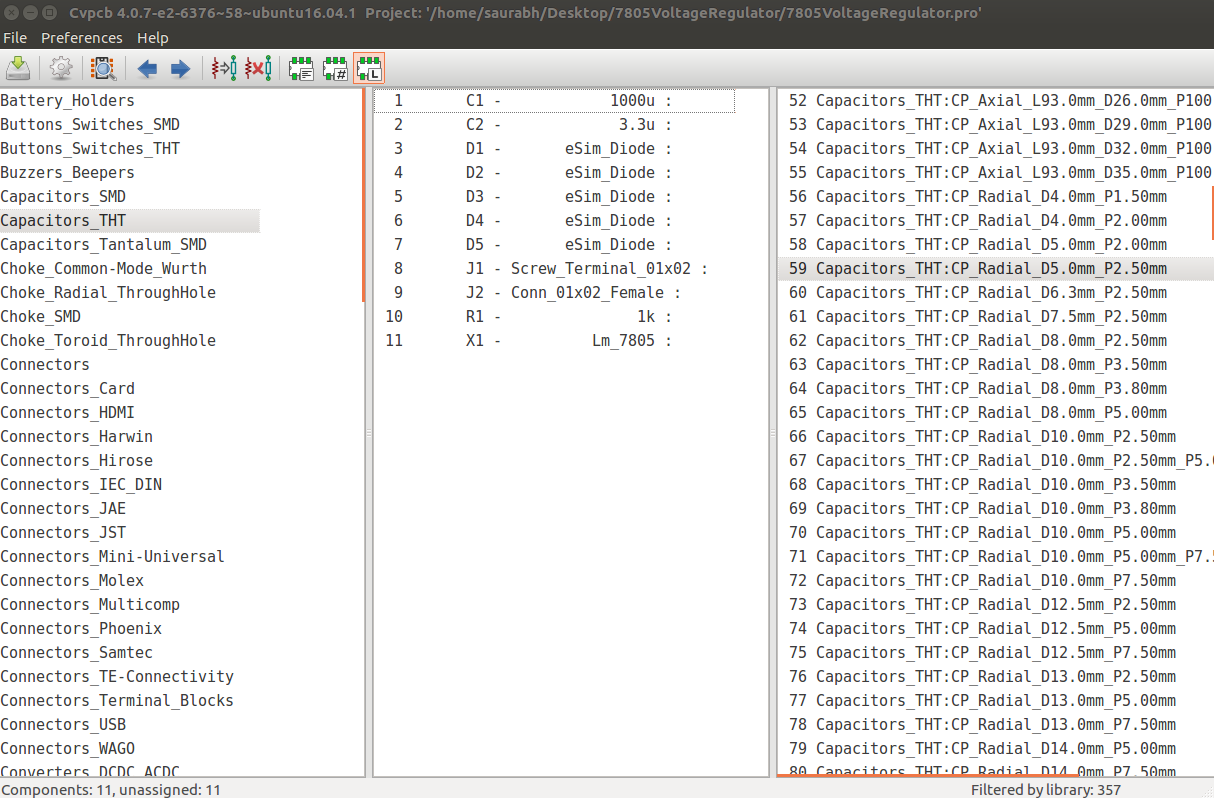
\includegraphics[width=\lgfig]{smnew.png}
\caption{Viewing footprint for C1}
\label{sm}
\end{figure}

\item Click on the \texttt{3D Display} icon in the {\tt Footprint}
window, as shown in \figref{2dview}. A top view of the selected footprint
in 3D is obtained. Click on the footprint and rotate it using the computer mouse to
get 3D views from various angles. One such view of the footprint
in 3D is shown in \figref{3dv}.

\end{itemize}

\begin{figure}
\centering
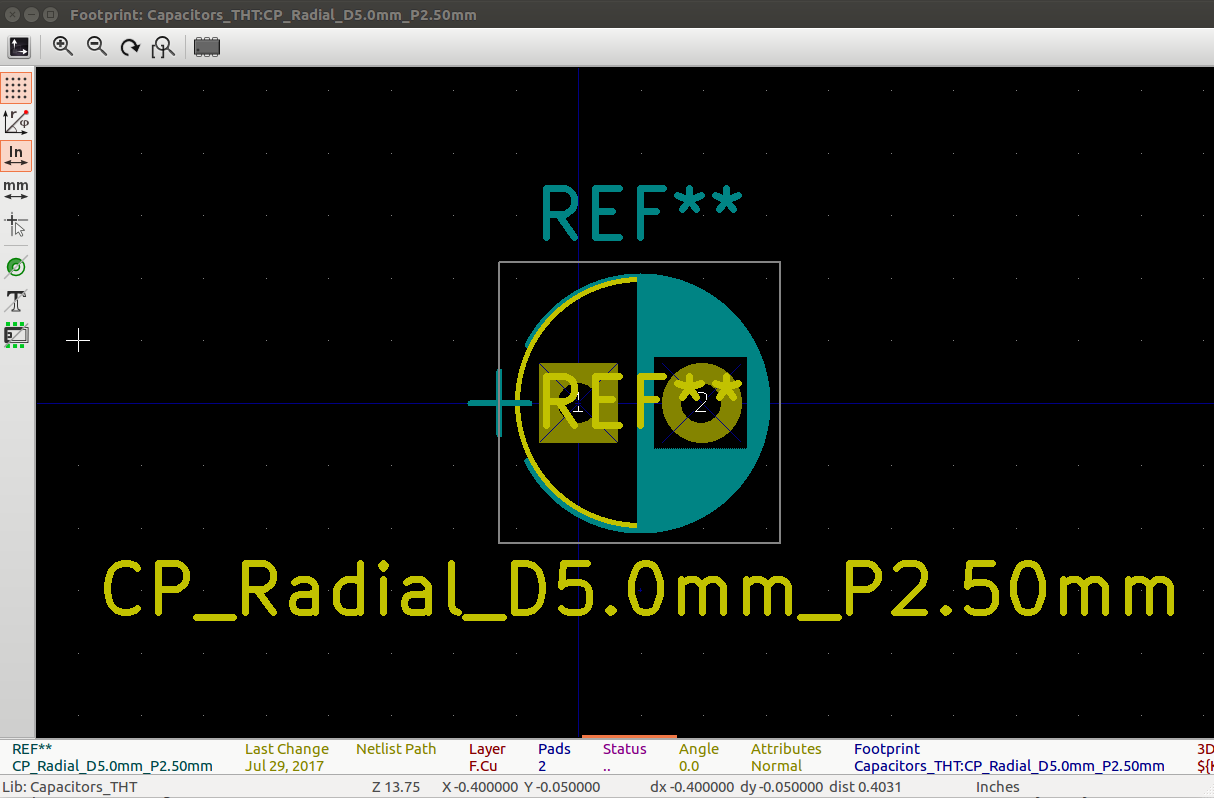
\includegraphics[width=\lgfig]{manual_images/2dviewofcp.png}
\caption{Footprint \texttt{CP\_Radial\_D5.0mm\_P2.50mm}'s view in 2D.}
\label{2dview}
\end{figure}
\begin{figure}
\centering
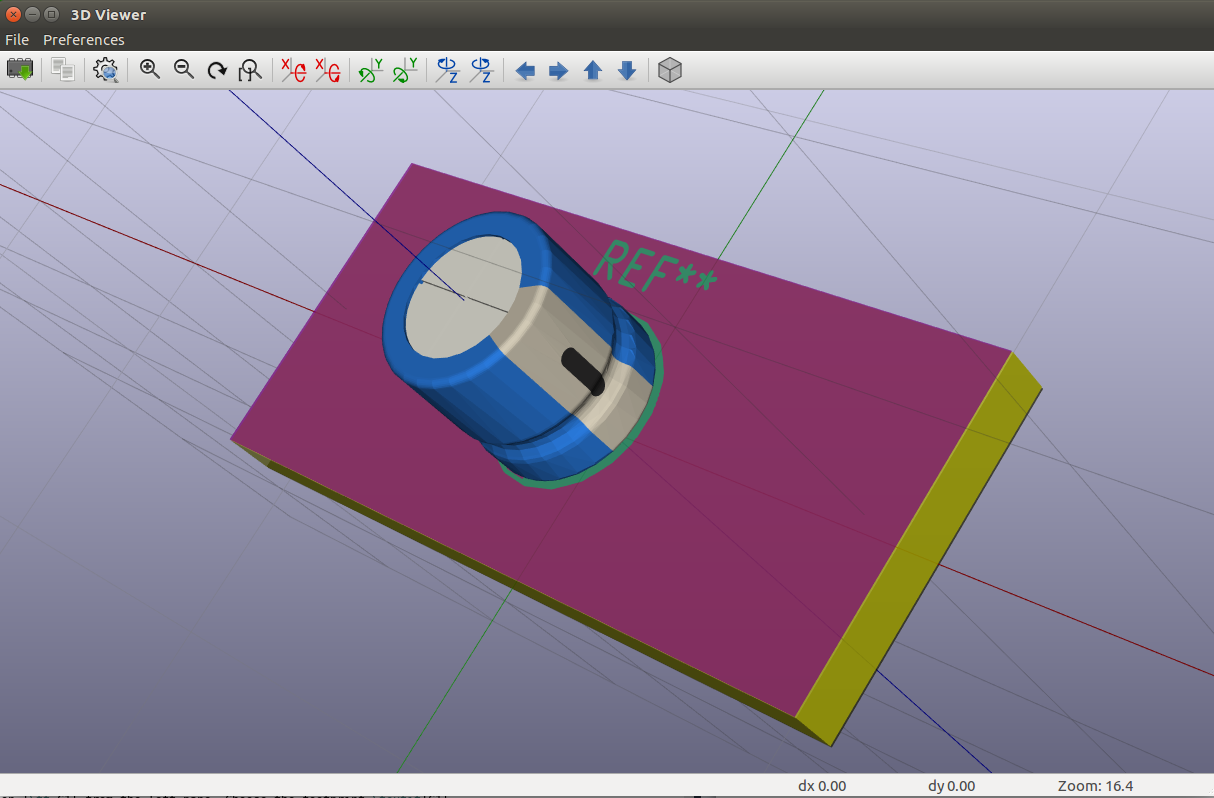
\includegraphics[width=\lgfig]{manual_images/3dv.png}
\caption{3D view of the footprint}
\label{3dv}
\end{figure}

\subsection{Mapping of components in the circuit}

\begin{compactenum}
\item Click on {\tt C1} from the middle pane. Choose the footprint  library \textit{Capacitors\_THT}
from the left pane and locate the footprint \linebreak \texttt{CP\_Radial\_D5.0mm\_P2.50mm}. By double clicking on it, the said footprint will be assigned to {\tt C1}.
\item Similarly choose the footprints per \figref{map} where the footprint association for all the footprints is shown in \figref{map}. Save the footprint association by clicking on the
\texttt{Save footprint association in schematic component footprint fields} tool from the {\tt CvPcb toolbar}. 
\end{compactenum}


\begin{figure}
\centering
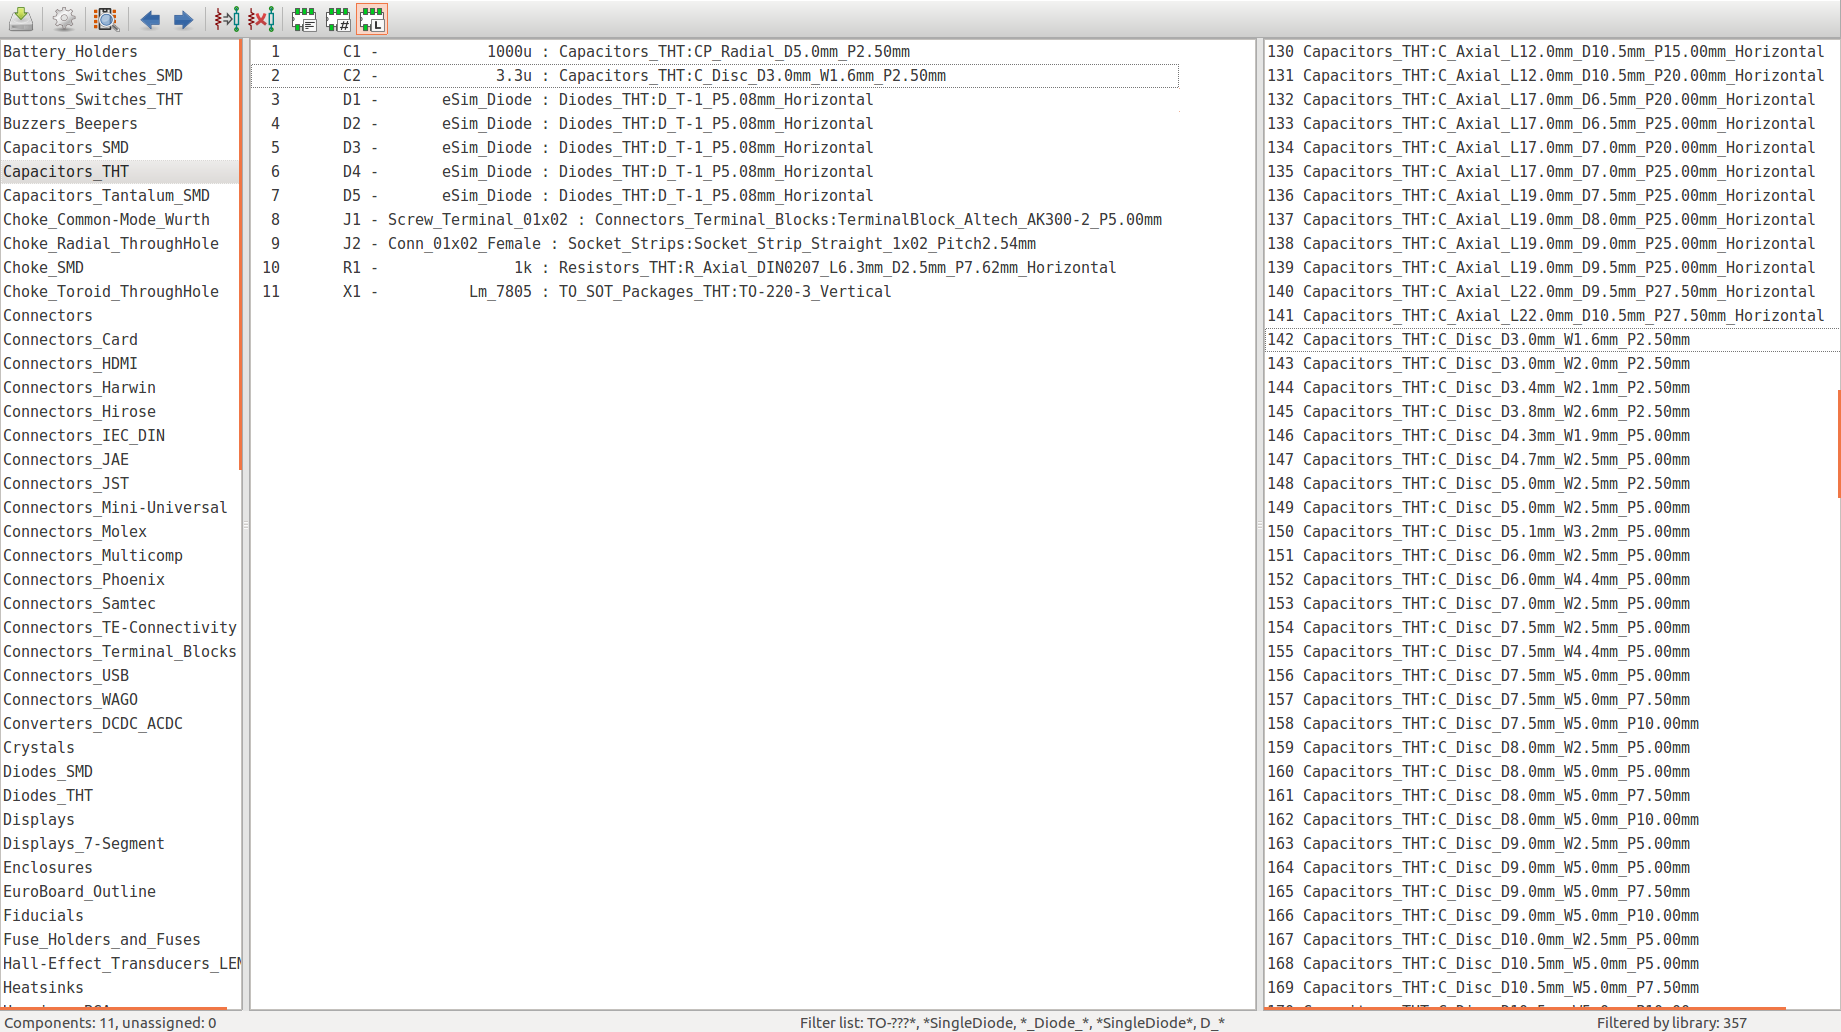
\includegraphics[width=0.85\linewidth]{manual_images/map.png}
\caption{Footprint mapping completed for the circuit}
\label{map}
\end{figure}.

\subsection{Netlist generation for PCB}
\index{Netlist!for PCB} \index{Netlist} 
\label{netc}
\begin{figure}
\centering
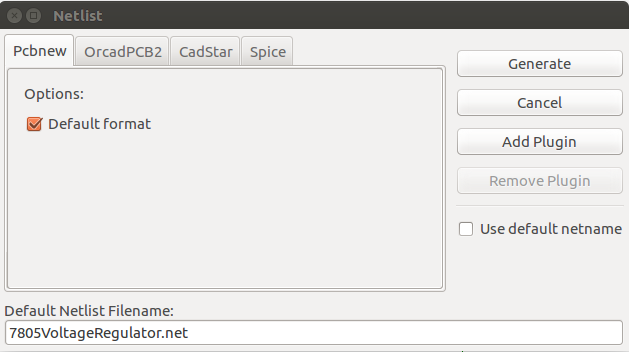
\includegraphics[width=\lgfig]{manual_images/netlistpcb.png}
\caption{Netlist generation for PCB}
\label{netlistpcb}
\end{figure}   

\begin{compactenum}
\item After having saved your footprint association, switch back to the Eeschema window and press Ctrl+S.
\item The netlist for PCB is different from that for simulation. To generate
netlist for PCB, click on the \textit{Generate netlist} tool from the
top toolbar in Schematic editor.
\item In the \texttt{Netlist} window, under the tab \textit{Pcbnew}, Select the option \texttt{Default format}. This is shown in \figref{netlistpcb}. Click on \texttt{Generate} option. 
\item Click on \texttt{Save} in the Save netlist file dialog box that opens up. Do not change the directory or the name of the netlist file. \texttt{Note that the netlist for PCB has an extension \emph{.net}. The netlist created for simulation has an extension \emph .cir}.
\end{compactenum}



\section{Creation of PCB layout}
\index{PCB Layout!creation} \index{Layout Editor}

The next step is to place the footprints and lay tracks between them
to get the layout. This is done using the \textit{Layout Editor}
tool. eSim uses {\tt Pcbnew}, the layout creation tool in KiCad, as
its layout editor.

\subsection{Launching Pcbnew}
\begin{compactenum}
\item To Launch the layout editor, \texttt{Pcbnew}, click on the \texttt{Run Pcbnew to layout printed circuit board} icon on the top right corner of the Schematic window.
\item Similarly, you can also click on \texttt{Tools}, and select the \texttt{Layout printed circuit board} option.
\item After doing either of the steps above, click \textbf{yes} on the \textit{Confirmation Box} that will appear on the screen.
\end{compactenum}

\subsection{Familiarizing the Layout Editor tool}
\index{Layout Editor}

The layout editor with the various menu bar and toolbars is shown in
\figref{pcbnew}.
\begin{figure}
\centering
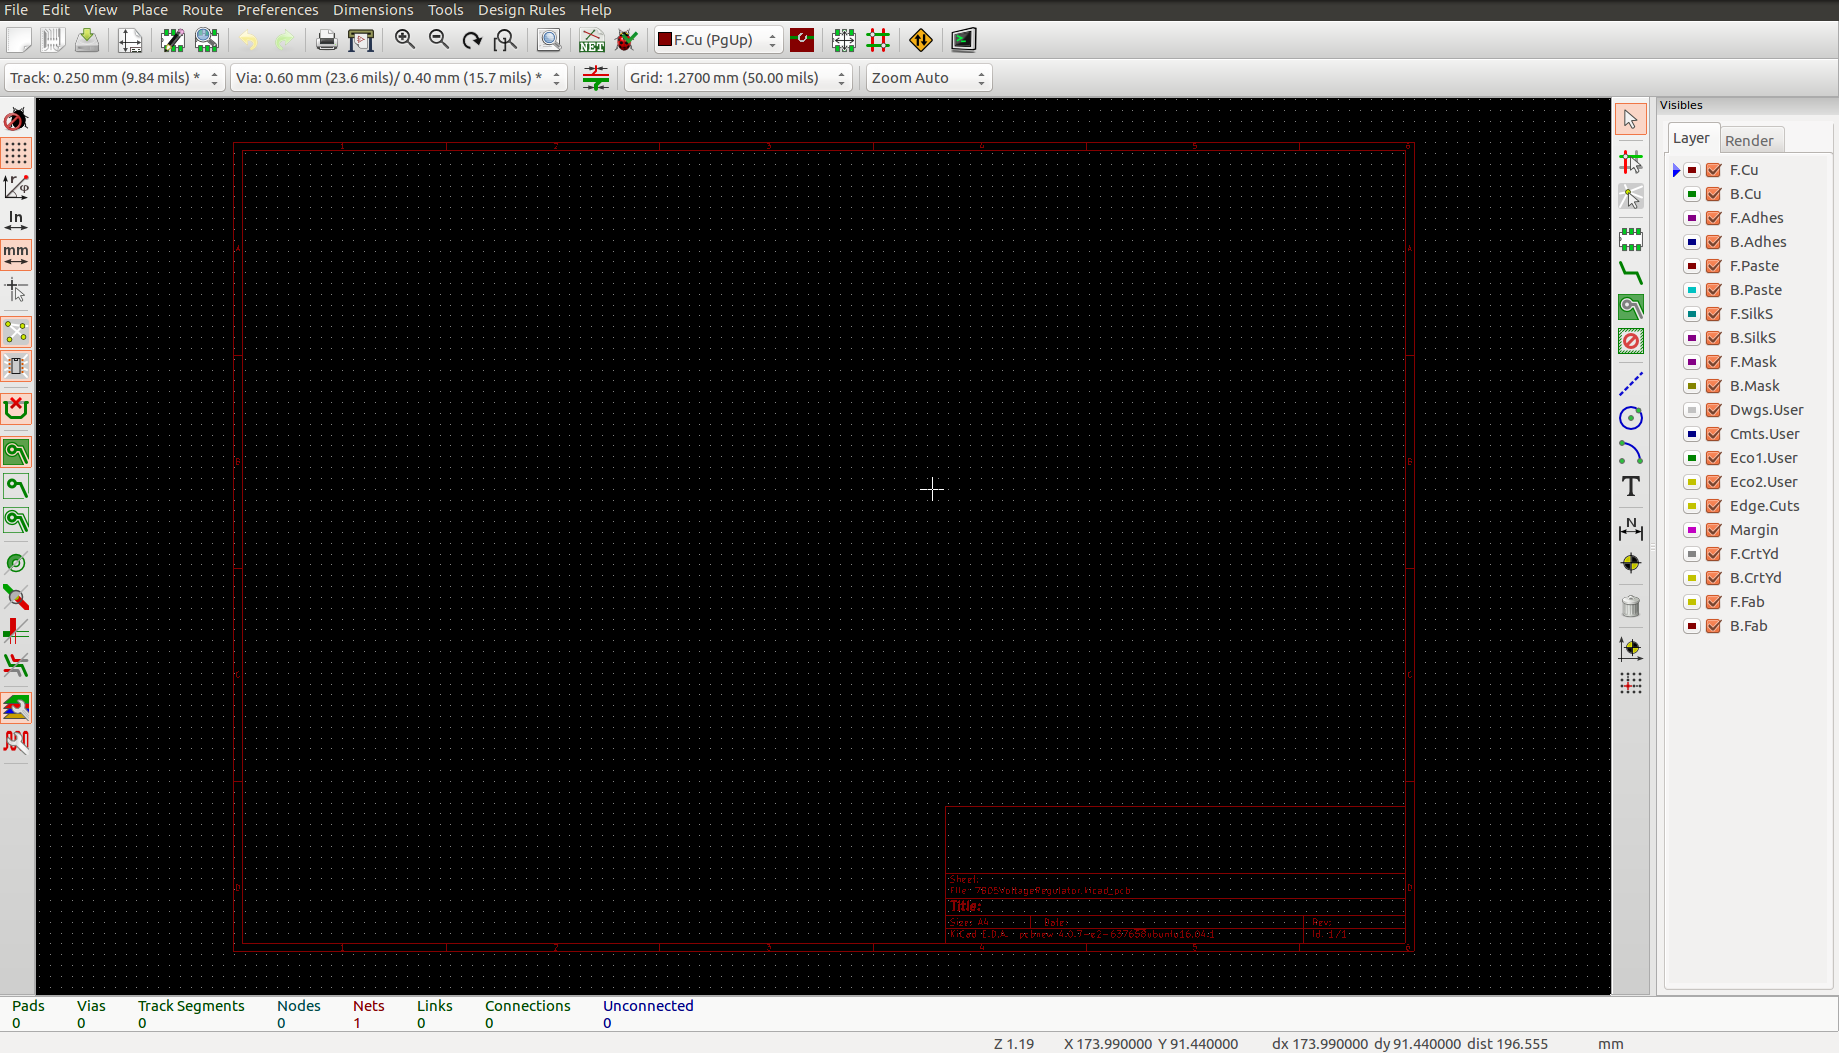
\includegraphics[width=0.68\linewidth]{NGHDL/toptble.png}
\caption{Layout editor with menu bar, toolbars and layer options}
\label{pcbnew}
\end{figure}


\subsubsection{Top toolbar}
Some of the important menu options in the top menu bar are shown in
\figref{pcbnew}. They are explained below:
\begin{compactenum}
\item Save board - Save the printed circuit board
%\item Module editor - Open module editor to edit footprint modules or
 % libraries
 \item Plot - This enables users to import their design in Gerber, PDF, SVG and few more formats depending on the requirement.
\item Read netlist - Import the netlist whose layout needs to be
  created.
\item Perform design rules check - Check for design rules, unconnected
  nets, etc., in the layout.
\item Select working layer - Selection of working layer.\\
Note: Selection of working layer can also be done from the \texttt{Layers toolbar} on the right-most side of the Pcbnew tool window.
\end{compactenum} 

\subsection{Hotkeys}
\index{Hotkeys!Layout editor}
A list of few important hotkeys is given below:
\begin{compactenum}
\item F1 - Zoom in
\item F2 - Zoom out
\item Delete - Delete Track or Footprint
\item X - Add new track
\item V - Add Via
\item M - Move Item
\item F - Flip Footprint
\item R - Rotate Item
\item G - Drag Footprint
\item Ctrl+Z - Undo
\item E - Edit Item
\end{compactenum}
The entire list of Hotkeys can be viewed by selecting \textit{Preferences} from the top
menu bar and choosing \textit{List Current Keys} from the option \textit{Hotkeys}.
\begin{figure}
\centering
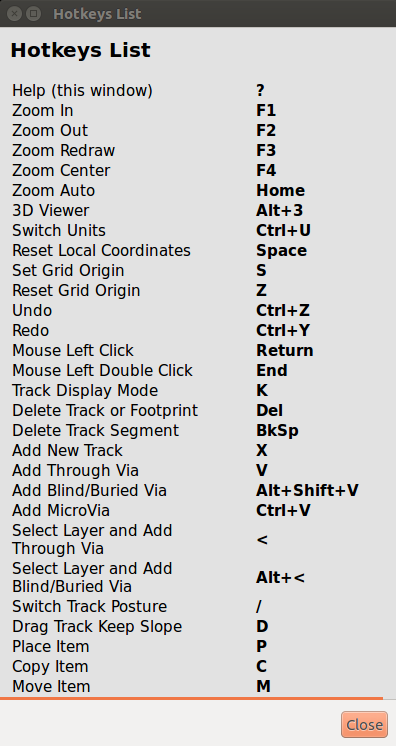
\includegraphics[height=0.4\textwidth]{manual_images/hotkeys.png}
\caption{Default Hotkeys}
\label{netlisttop}
\end{figure}
%[width=0.5\textwidth]

\subsection{Designing PCB layout for 7805VoltageRegulator circuit} \index{PCB design}
Click on \textit{Read Netlist} tool from the top toolbar of Pcbnew. Click on
\textit{Browse Netlist files} on the Netlist window that opens
up. Select the {\tt .net} file that was modified \\\texttt{after}
assigning footprints. Click on \textit{Open}. Now Click on
\textit{Read Current Netlist} on the Netlist window. The
sequence of operations is shown in \figref{brnet}. 
\index{PCB design!move modules} \index{PCB design!lay tracks}

\begin{figure}
\centering
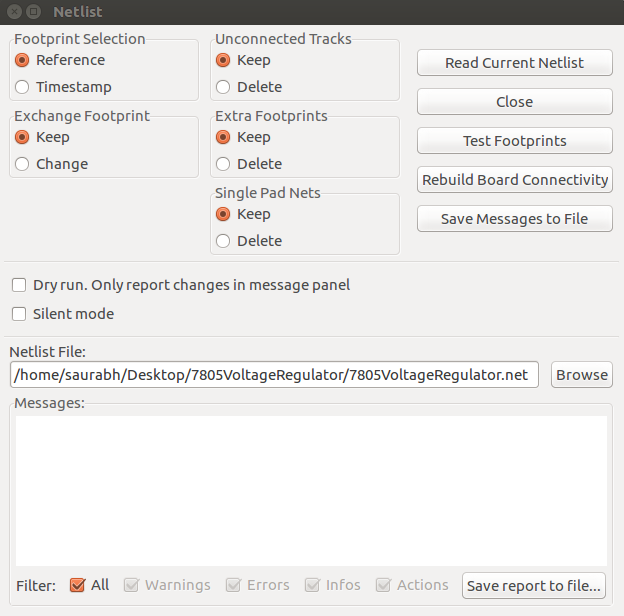
\includegraphics[width=0.67\linewidth]{manual_images/readnetlist.png}
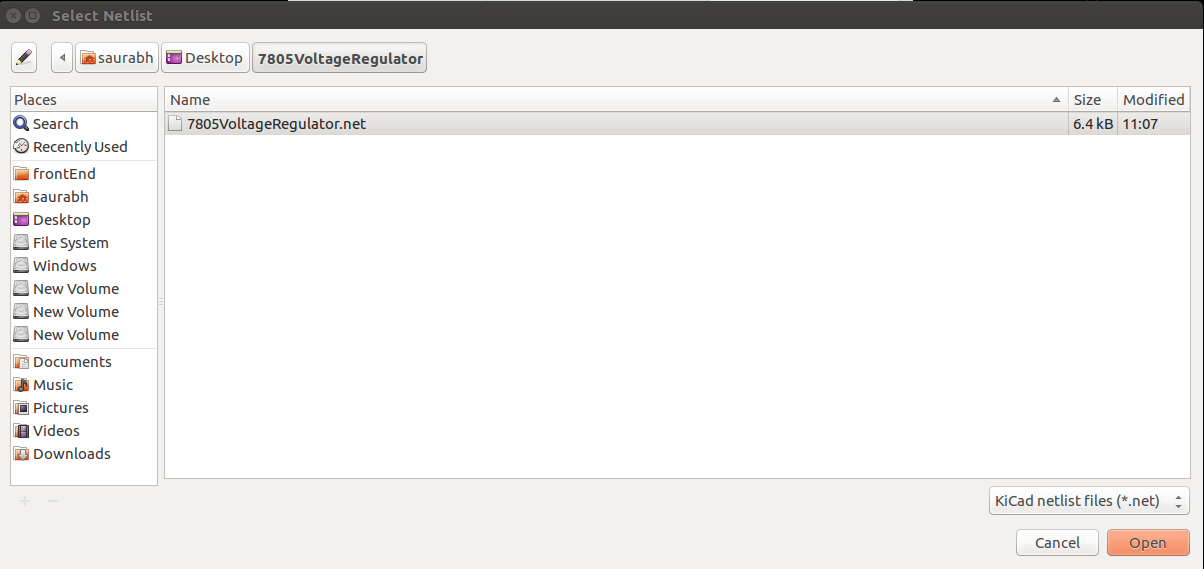
\includegraphics[width=0.67\textwidth]{manual_images/browsenetlistforpcb.png}
\caption{Importing netlist file to layout editor: 1. Browse netlist
  Files, 2. Choose the appropriate .net file, 3. Read Netlist file, 4. Close}
\label{brnet}
\end{figure} 
 
\subsubsection{Arranging the footprints}
\begin{compactenum}
\item After clicking on Read Netlist button and closing the Read Netlist window, the footprints that we assigned will appear on the Pcbnew screen in a cluttered fashion, stacked on top of each other as shown in \figref{cluttered}
\begin{figure}
\centering
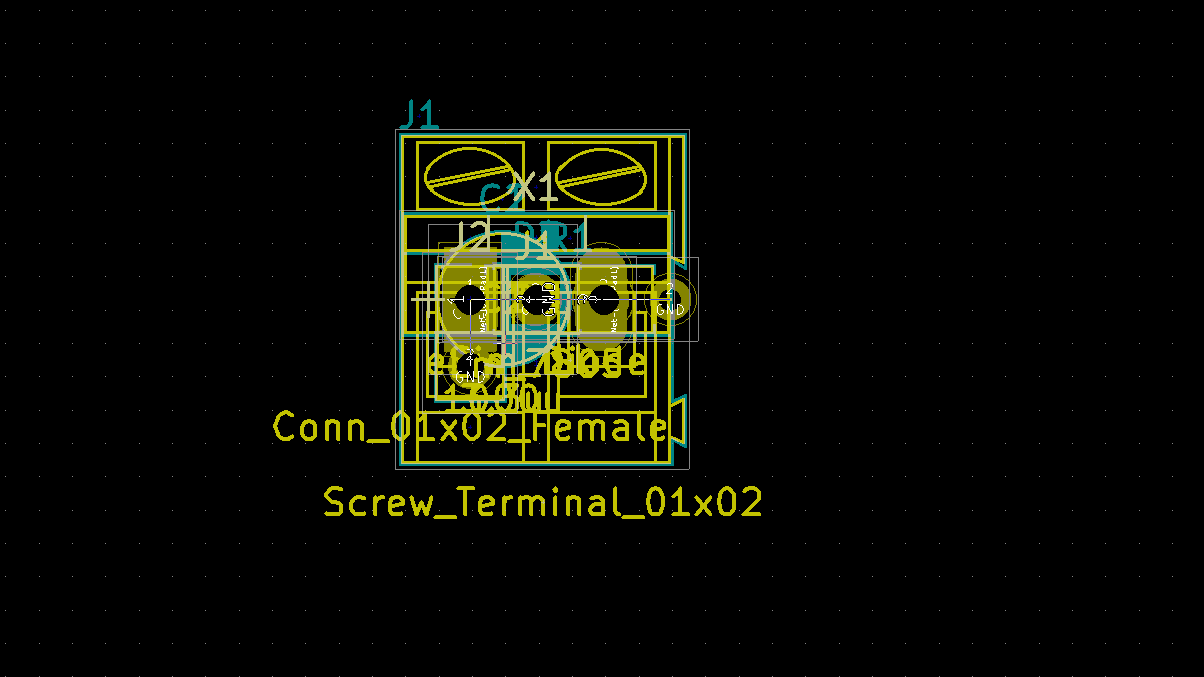
\includegraphics[height=0.4\textwidth]{cluterredFPs.png}
\caption{Cluttered footprints}
\label{cluttered}
\end{figure}

\item Let us separate these footprints and place them in proper orientation per the requirement of the circuit. Let us start with Screw\_Terminal\_01x02 footprint.
\item Right Click on the text \texttt{Screw\_Terminal\_01x02} in the Pcbnew window, and select \texttt{Footprint J1 on F.Cu.} and select the \texttt{Move} option from the list.
\item The footprint will be glued to the cursor and it can be placed in the location of one's choice by moving the cursor at the desired location and clicking once to place it there.
\begin{figure}
\centering
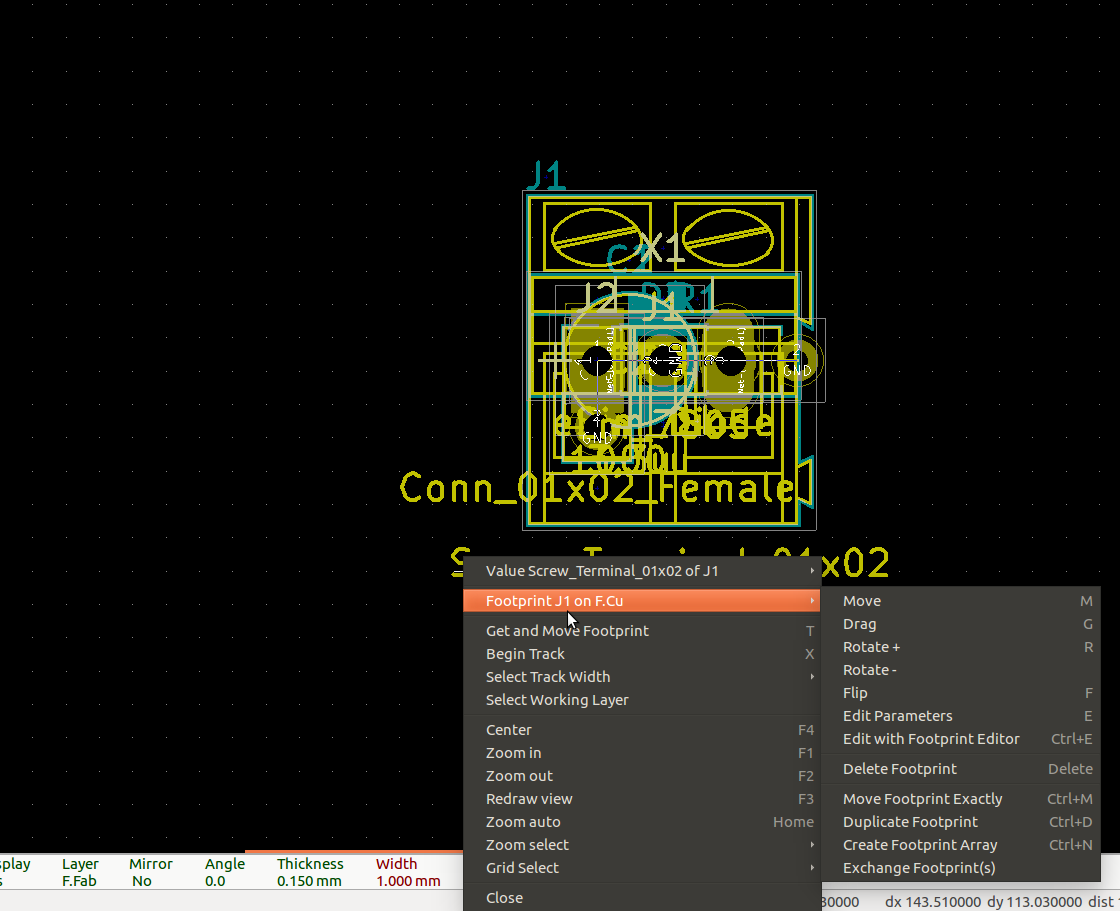
\includegraphics[height=0.4\textwidth]{FPMove.png}
\caption{Moving the footprint}
\label{movingFP}
\end{figure}
\item We have moved the Screw\_Terminal\_01x02 footprint to the left side of the Pcbnew window.
\item Once again right click on the text \texttt{Screw\_Terminal\_01x02} in the Pcbnew window, and select \texttt{Footprint J1 on F.Cu.} and select the \texttt{Rotate +} option from the list as shown in \figref{rotateFP}
\begin{figure}
\centering
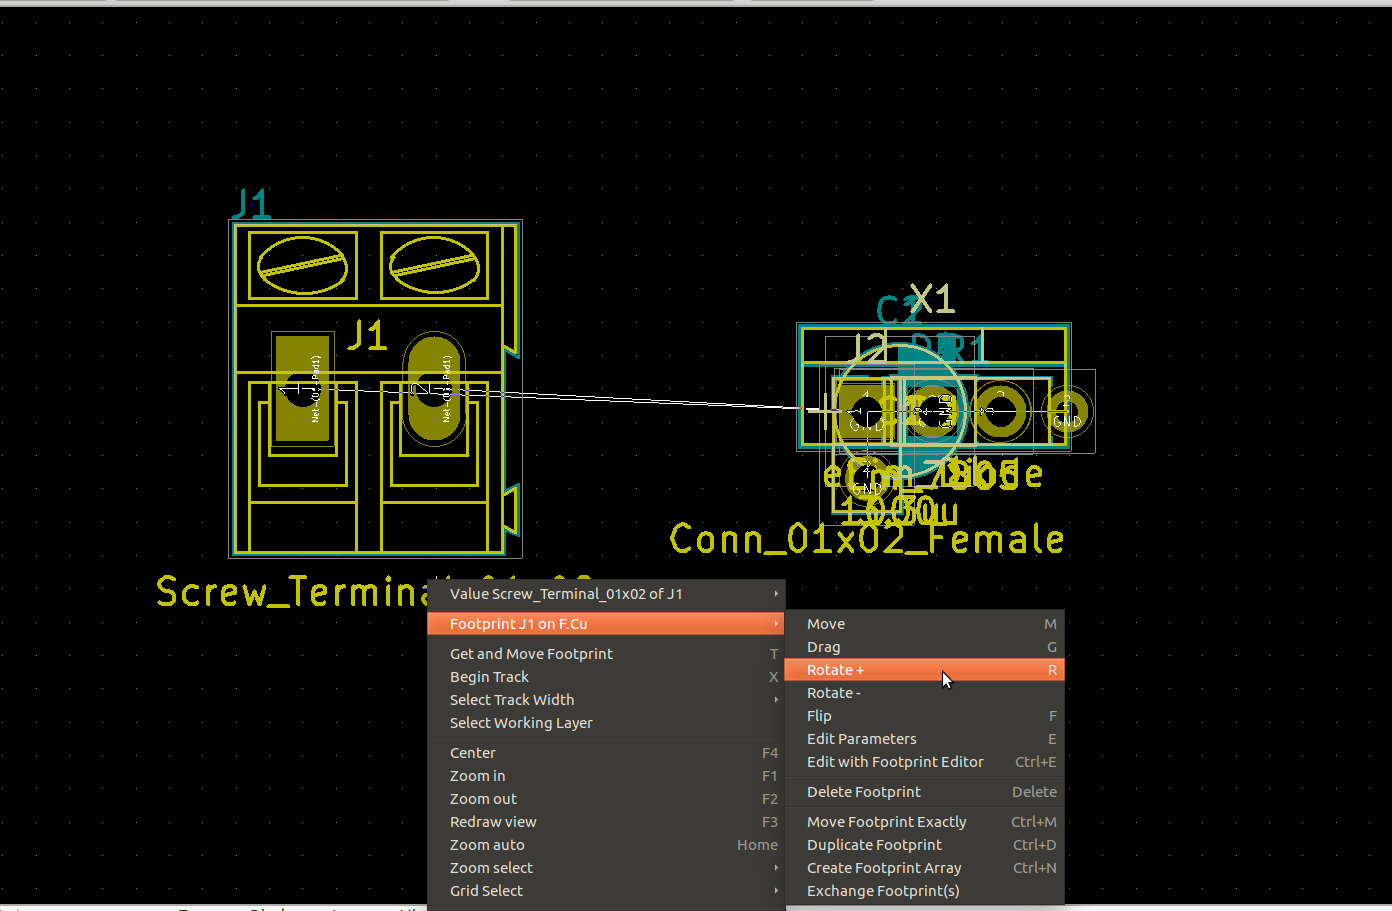
\includegraphics[height=0.4\textwidth]{rotatefp.png}
\caption{Rotating the footprint}
\label{rotateFP}
\end{figure}
\item Using similar methods, we have moved and rotated all other footprints as shown in \figref{rotateall}

\begin{figure}
\centering
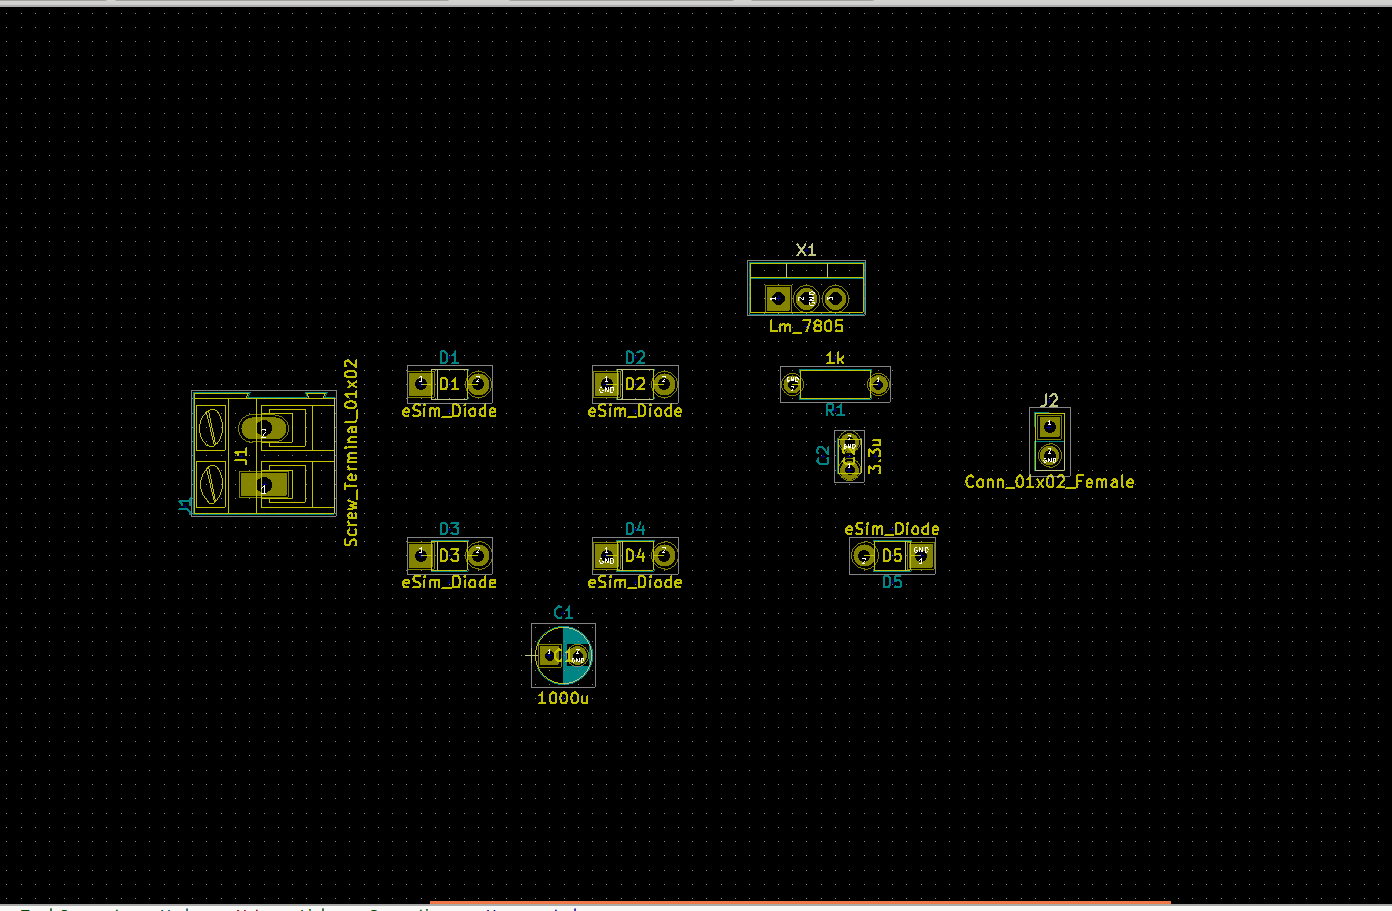
\includegraphics[height=0.4\textwidth]{fpsmovedandrotated.png}
\caption{All footprints moved and rotated}
\label{rotateall}
\end{figure}
\end{compactenum}

\subsubsection{Setting Design Rules}

\begin{compactenum}
\item Click on \texttt{Design Rules on top of the Pcbnew window, select Design Rules option from the drop down menu there.}
\item \texttt{Design Rules Editor} window will open, Under the \texttt{Net Classes Editor}, locate the \texttt{Track Width} box, erase the default value from the window placed under the \texttt{Track Width} box and enter 1.25 as the track width.
\item Click on \texttt{Global Design Rules}, under Minimum Allowed Values, locate \texttt{Min track width}, erase the default value and enter 1.25 in the data entry field on the right side of it as shown in \figref{DRC_GDR}. This will ensure that all tracks placed are of width 1.25mm and that when we perform Design Rules Check, the checks will be made such that all tracks are of the width 1.25mm will be checked.
\item Click on Ok button and close the Design Editor Rules window.
\end{compactenum}

\begin{figure}
\centering
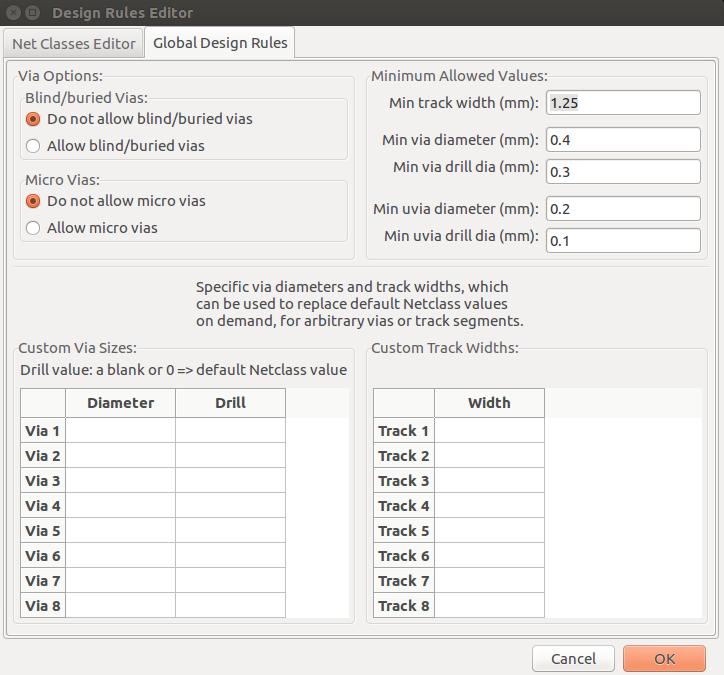
\includegraphics[height=0.4\textwidth]{druleseditor.png}
\caption{Design Rules Editor Window: Global Design Rules}
\label{DRC_GDR}
\end{figure}

\subsubsection{Drawing the Board Outline}
\begin{compactenum}
\item Board outline defines the physical dimensions of your board. After the fabricator is done placing tracks and other processes, he/she will cut your design from the copper cladded sheet or the material used per your choice, as per your board outline dimensions. Say, if your board outline is of rectangular shape with dimensions 80mmx50mm, the fabricator will cut the copper sheet of the said dimension. Its important to know that all the tracks(physical electrically conductive connections between two nodes or points on a PCB) must lie inside this board outline.
\item We will also choose a board outline of rectangular shape. Select working layer as \texttt{Edge.Cuts} from the Layers menu on the far-right side of Pcbnew.
\item Click on \texttt{Place} from the top-left tool bar of the Pcbnew window and select \texttt{Line or Polygon}. A pencil icon will appear to be tied to the cursor.
\item Click once on the layout editor to start drawing the outline. Drag the cursor either horizontally or vertically. When it comes to the corner of the board, click once and drag the cursor in perpendicular direction. Do this till you reach the origin of the outline, and double click to finish drawing the rectangular outline. Completed outline is as shown in \figref{brdoutline}.
\end{compactenum}

\begin{figure}
\centering
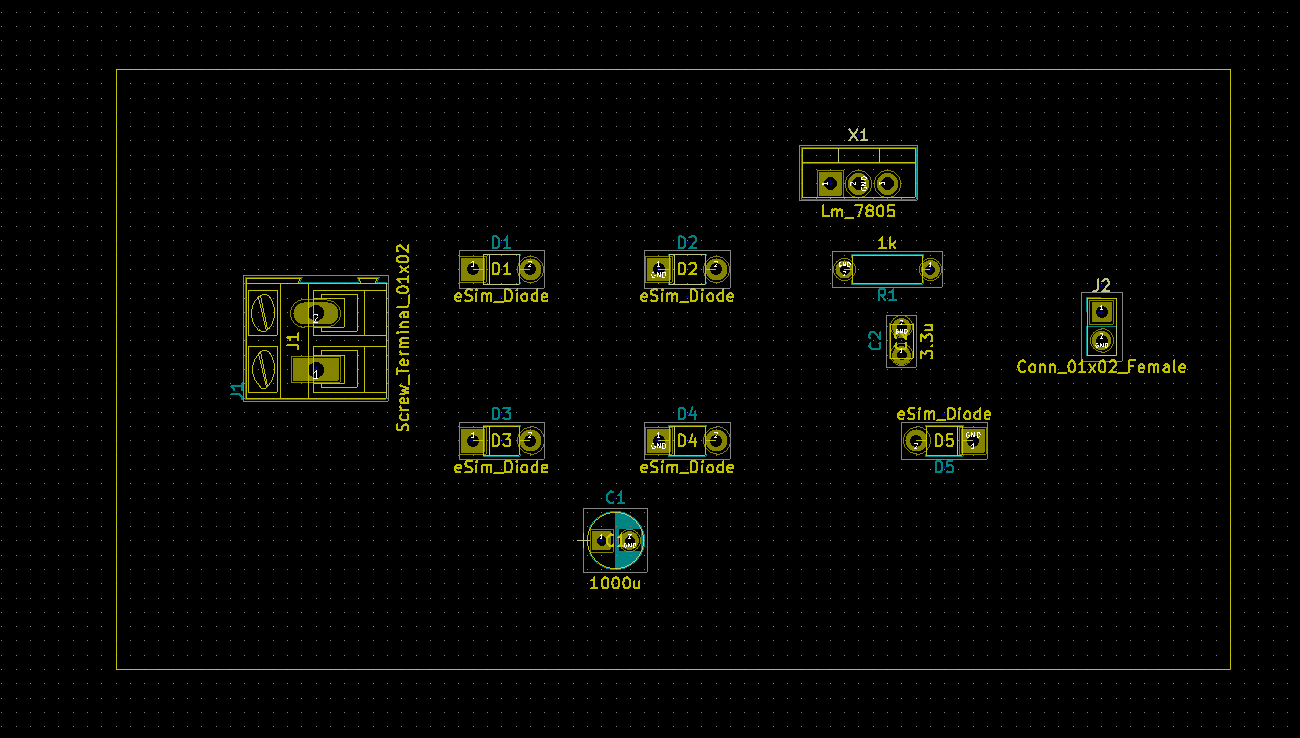
\includegraphics[height=0.4\textwidth]{boardoutline.png}
\caption{Drawing a board outline}
\label{brdoutline}
\end{figure}

\subsubsection{Placing Tracks}
\begin{compactenum}
\item Select the working layer as B.Cu from the Layers menu on the far-right side of Pcbnew.
\item Click on \texttt{Place} from the top-left tool bar of the Pcbnew window and select \texttt{Track}. A pencil icon will appear to be tied to the cursor.
\item The procedure to place a track between Node 2 of Screw\_Terminal\_01x02 to Node 1 of D3 diode, as shown in \figref{brdoutline} is described in below steps.
\item Working layer is B.Cu., \texttt{Place Track tool} is selected earlier. Click the pencil icon tied to cursor on the Node 2 of Screw\_Terminal\_01x02 and drag the cursor till Node 1 of D3 diode and double click on Node 2 of D3. By double clicking the track will end at Node 2 of D3. Please refer \figref{D3node1track} for the mentioned track being placed.
\begin{figure}
\centering
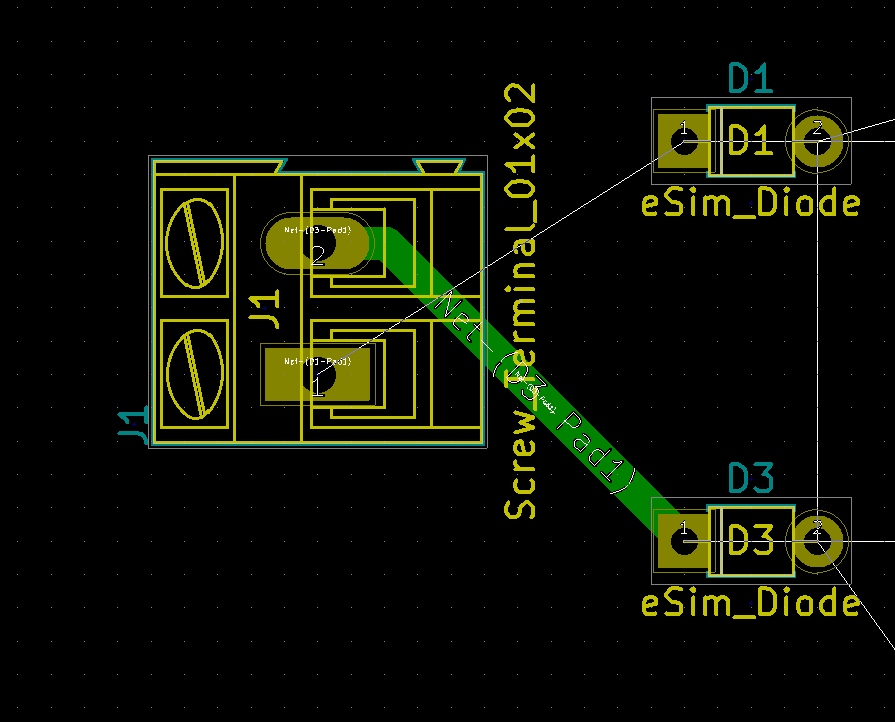
\includegraphics[height=0.4\textwidth]{firsttrack.png}
\caption{Track placed on B.Cu. between Screw\_Terminal\_01x02 connector and D3 Diode}
\label{D3node1track}
\end{figure}
\item Similarly, all the tracks have been placed as shown in \figref{alltracks}. Please note that tracks shown in green color are on B.Cu. layer whereas the tracks in red color are placed on the F.Cu. layer. 
\begin{figure}
\centering
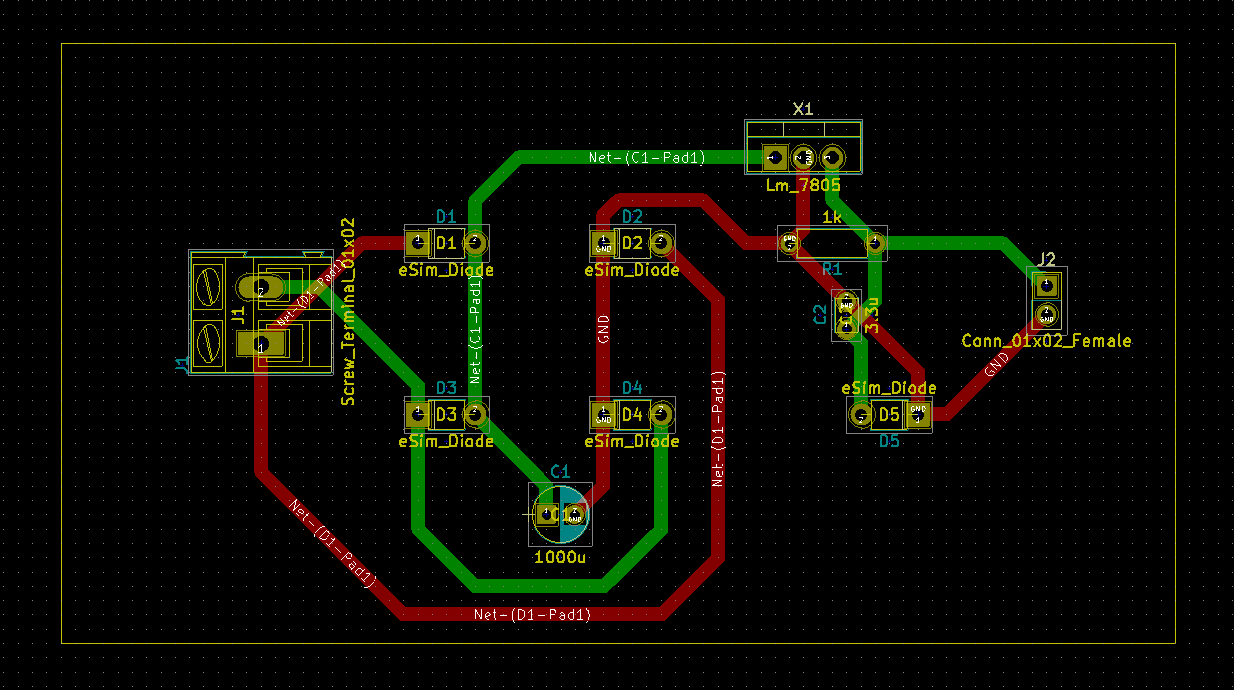
\includegraphics[height=0.4\textwidth]{alltracks.png}
\caption{All tracks placed}
\label{alltracks}
\end{figure}
\end{compactenum}

\subsubsection{Performing Design Rules Check(DRC)}
\begin{compactenum}
\item After tracks are placed, it is important that the design created by used should not violate any design rules set earlier.
\item Click on \texttt{Perform Design Rules check} button from the top menu bar of Pcbnew. DRC Control Window will pop-up as shown in \figref{DRC}.
\item Click on \texttt{Start DRC}, and observe if any messages/warnings appear in the \texttt{error messages} window at the bottom of the DRC Control window. If there are no errors in the design present, there will not be any errors in the message window as shown in \figref{DRC}
\end{compactenum}

\begin{figure}
\centering
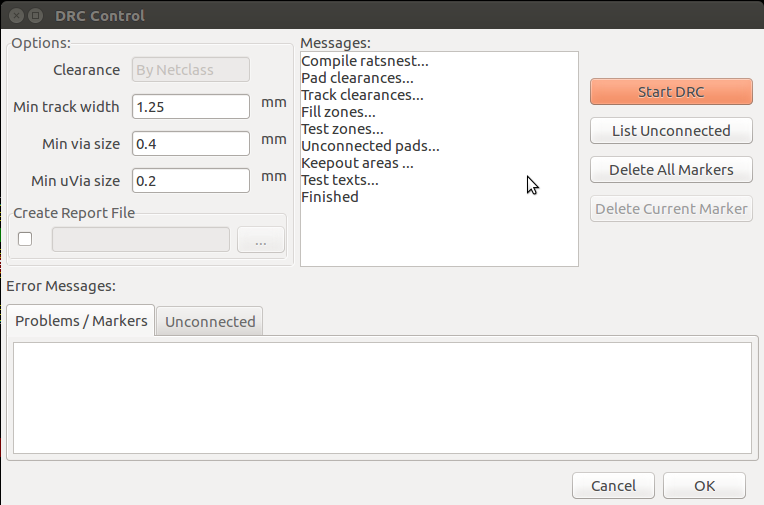
\includegraphics[height=0.4\textwidth]{drc1.png}
\caption{DRC Control Window}
\label{DRC}
\end{figure}

\subsubsection{Exporting the Design to Gerber format}
\begin{compactenum}
\item Click on \texttt{Plot} tool from the top toolbar, select the Plot Format as \texttt{gerber} from the drop down menu of Plot Format.
\item Select the directory in which the user wishes to save the gerber files. 
\item Select F.Cu, B.Cu, B.Silks, F.Mask, B.Mask, Margin and Edge.Cuts from the \textit{Layers} on the left side of the Plot window as shown in \figref{plotbef}.
\item After clicking on 'Plot' button, acknowledgment messages can be seen in the 'Messages' window at the bottom of the \texttt{Plot} tool window as shown in \figref{plotaf}.
\end{compactenum}


\begin{figure}
\centering
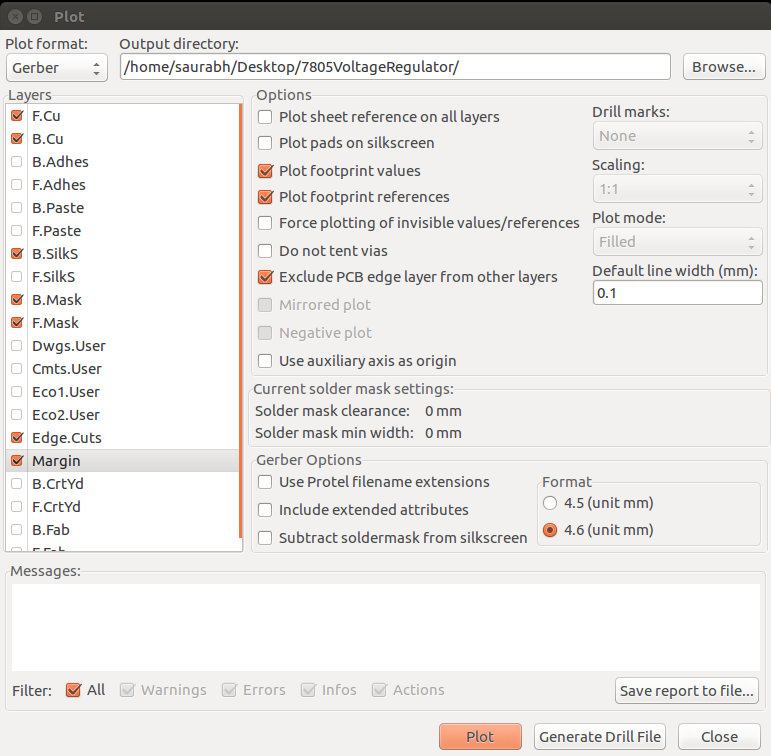
\includegraphics[height=0.4\textwidth]{plotwindowbefore.png}
\caption{Plot Window before generating gerber files}
\label{plotbef}
\end{figure}

\begin{figure}
\centering
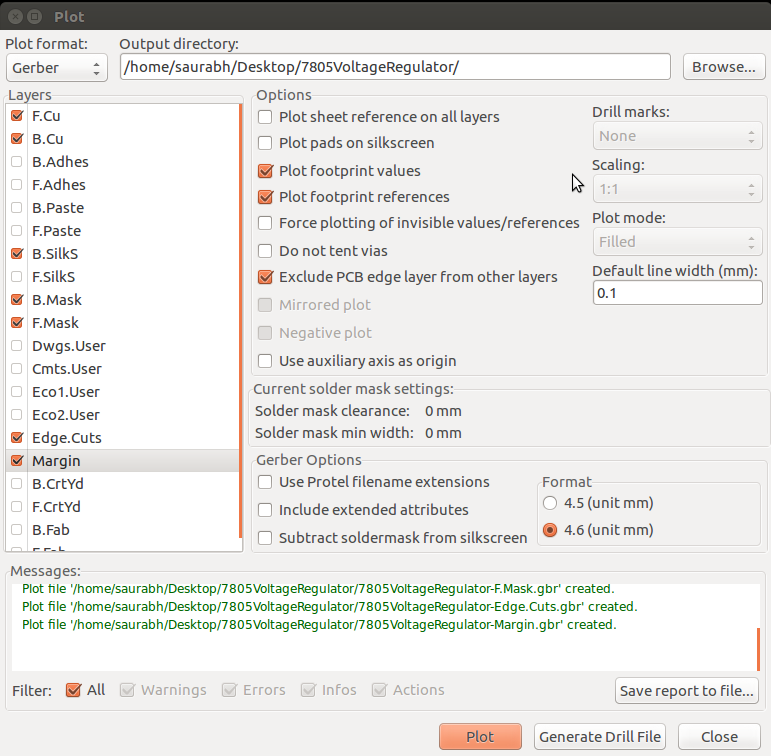
\includegraphics[height=0.4\textwidth]{plotafter.png}
\caption{Plot window after generating gerber files}
\label{plotaf}
\end{figure}

\subsubsection{Viewing the Gerber files generated}
\begin{compactenum}
\item Open the terminal by Ctrl+Alt+T keys, and type \texttt{gerbview} and press enter. Gerbview tool of KiCad will open up. For windows OS users, search for \texttt{gerbview} application through Windows' search application option.
\item Click on File from top-left menu, and select Load Gerber File option.
\item Go to the directory where you have stored the earlier created gerber files as shown in \figref{gerbviewloading} and click on Open.
\item The design created earlier will appear in the gerbview window as shown in \figref{gerbviewcapture}.
\end{compactenum}

\begin{figure}
\centering
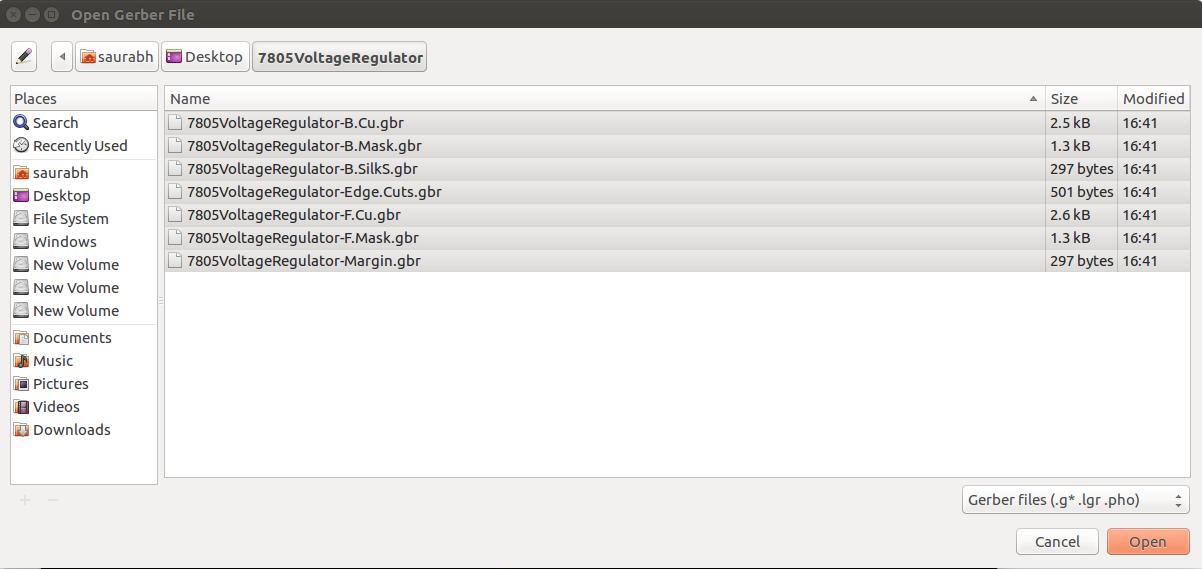
\includegraphics[height=0.4\textwidth]{gerbviewloading.png}
\caption{Loading gerber files in the gerbview}
\label{gerbviewloading}
\end{figure}

\begin{figure}
\centering
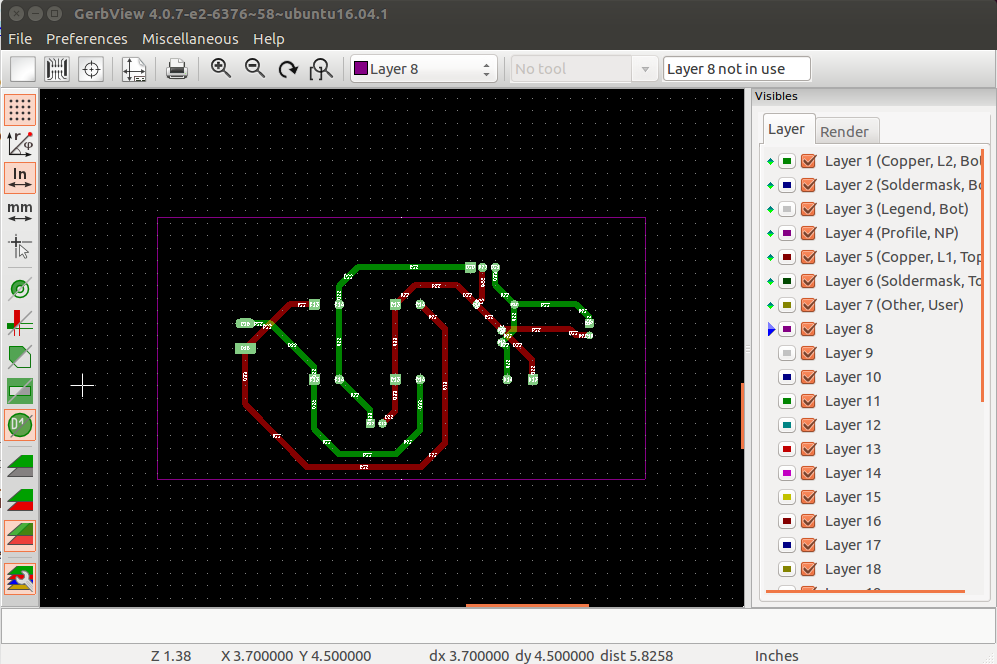
\includegraphics[height=0.4\textwidth]{gerbviewcapture.png}
\caption{Observing the design in Gerber format}
\label{gerbviewcapture}
\end{figure}